%----------------------------------------------------------------------------
\chapter{A hálózat vizsgálatának lépései}
%----------------------------------------------------------------------------
A hálózat vizsgálatát több részre osztottam, mivel különböző programozási nyelveket használtam az eredmények kimutatásához.

Az alábbi ábra szemlélteti a kutatási folyamat lépéseit:


\begin{figure}[h]
	\centering
	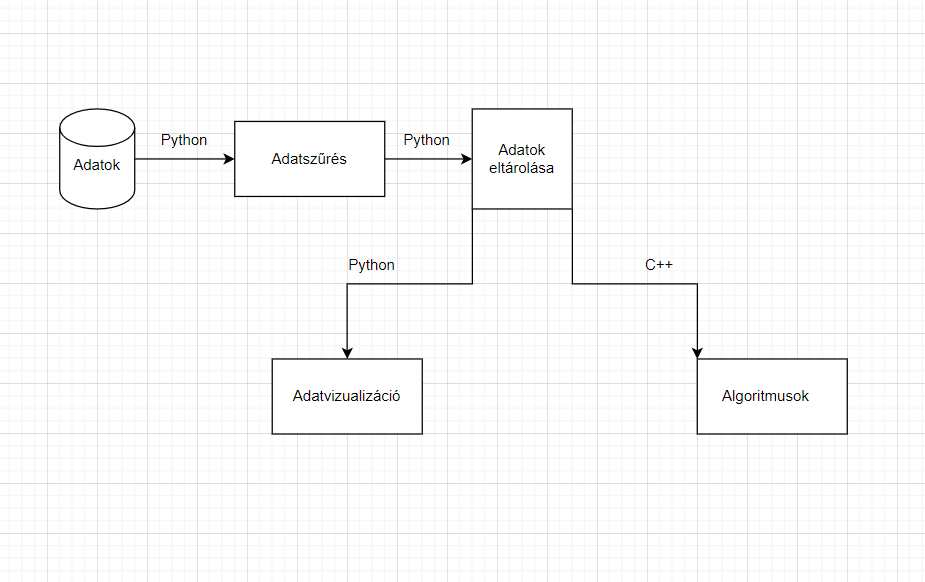
\includegraphics[scale=0.7]{images/lepesek}
	\caption{Folyamat ábra}
\end{figure}
\begin{itemize}
    \item Első lépésként az adatszűrés , adatbányászat , amely következtében feldolgozható adatokat átállítottam elő és ezen lépés után két részre választottam a műveleteket.
    \item  Egyik rész az adatok vizualizációja. Itt kirajzolásra kerül a hálózat kis rész gráfja és annak fejlődése .
    \item Második részben pedig a gráfelméletben megjelenő szociális jelenségek vizsgálata és ahhoz köthető algoritmusok megírása volt a fő célpont.
\end{itemize}
 
A programozási nyelvekek közül két különböző nyelvet, Python-t és C++-ot választottam, és használtam az adatokkal való műveletek és vizsgálatok során. A Python egy interpretált nyelv, ami azt jelenti, hogy fordítás nélkül futtatható. Ezzel szemben a C++ nyelvű forráskódot gépi kóddá kell fordítani a futtatható állomány létrehozása érdekében. A Python dinamikusan típusos nyelv, ami azt jelenti, hogy a változók típusát futásidőben határozza meg, nem kell előre meghatároznunk. Ez a tulajdonság nem alkalmazható a C++ nyelvre, de érdemes megemlíteni, hogy a C++ egy hatékony nyelv, amely lehetővé teszi a hardverközeli programozást és a memóriakezelést precízen irányítja.

Miért választottam a Python és a C++ nyelveket a kutatás során? Először is, minden műveletet el lehetett volna végezni más nyelveken is. Például az adatokat adatbázisban tárolhatnánk és az adatbáziskezelő nyelvét, például SQL-t használhatnánk a műveletek végrehajtásához. Egy másik lehetőség az adatok feldolgozására és vizualizációjára az adatbázisból való lekérdezések segítségével. Azonban én a Python és a C++ nyelveket választottam, mert a gráfelméleti algoritmusokat C++ nyelven tanultam, amihez a diákok már korábban is kapnak betekintést középiskolai tanulmányaik során. Ezért egy olyan nyelvet választottam, amelyet már ismernek, és könnyen át tudják gondolni az algoritmusok lényegét, ahelyett, hogy egy új nyelvet kellene elsajátítaniuk a téma mellett.

Ezzel a döntéssel a diákoknak lehetőségük van jobban megérteni és követni a programozási részleteket, és könnyebben alkalmazni a gráfelméleti algoritmusokat a kutatás során.

\section {Adatbányászat, adatszűrés}


Az adatbányászathoz a Python nyelvet használtam, amely segítségével sikerült megszerezni az összes Enron cég által biztosított e-mail címet. Konkrétan 5653 e-mail cím van, amelyek "@enron.com" végződéssel rendelkeznek. A kommunikációs hálózat létrehozásához az üzenetek jelentik az építőelemet, tehát ki kellett bányásznom és el kellett mentenem az üzeneteket annak érdekében, hogy létrehozhassak egy gráfot, amelyet vizsgálhatok. A szűrés ebben az esetben fontos volt, hogy csak az Enron-os e-mailek közötti üzeneteket használjam fel, ezzel csökkentve az adatok méretét. Még így is rengeteg adatot kaptam, pontosan 88975 üzenetet, amelyekről csak a minimális információt (küldő, címzett és dátum) mentettem el.

\begin{figure}[h]
	\centering
	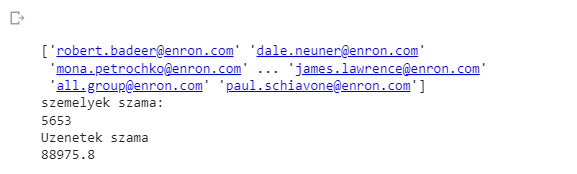
\includegraphics[scale=1]{images/adatokszama}
	\caption{Adatok számlálásának eredménye}
\end{figure}
\pagebreak%johet ide egy kodreszlet majd magyarazat  
 Az alábbi kódrészlettel kezdtem az adatokat kinyerni a megkapott adattömegből

\begin{figure}[h]
	\centering
	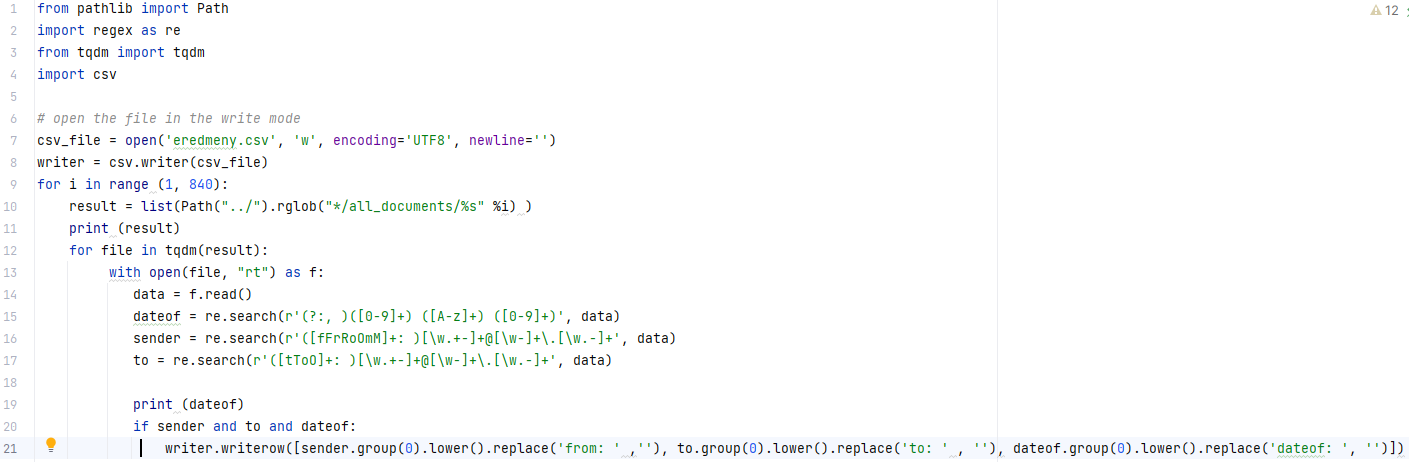
\includegraphics[scale=0.5]{images/adatbanyaszat}
	\caption{Adatbányászat}
\end{figure}

\begin{itemize}

        \item első lépésként létrehoztam egy csv fájlt, amelyben a megkapott adatokat tudom tárolni
	\item a következő lépés egy ciklus létrehozása, hogy minden személyt leellenőrizünk
	\item minden mappában több email szerepelt ezért először meghatároztam a fájlok listáját 
	\item ezen lista elemeit, tehát az összes fájlt meg kellett nyitnom és kikeresni a számomra szükséges adatokat(küldő,címzett és dátum)
	\item ezen adatok kiválasztásához regex kifejezéseket használtam amellyel nagyon egyszerűen lehetett rátaláni a helyes adatokra 
	\item minden olyan esetben ha volt dátum, küldő és címzett akkor az adathármast kiírattam a program elején létrehozott fájlba
        \item  ugyanakkor az itt kapott eredményt még át kellett futtatnom egy szűrési algoritmuson amelyet már az adatok biztonságos tárolása miatt Drive-ra töltöttem fel és onnan használtam fel .
         \item a szűréshez is Python nyelvet használtam amelyet már a gyors mentési lehetőséggel élve Colab-ban írtam meg.
         \item  a legfontosabb szempont az volt a helyes adatok kiválasztásában, hogy felhasználók e-mail címei "@enron.com"-végződéssel rendelkezzenek ugyanakkor az üzenetekben mindkét személyre jellemző legyen ezen tulajdonság.
\end{itemize}




\section {Adatvizualizáció}

A következő részben röviden bemutatom a hálózat megjelenítését és annak fejlődését.

Az ábrákon és adatokon, amelyeket eredményként bemutatok, az első 50 e-mail címet vettem figyelembe, valamint a közöttük lévő szigorú kapcsolatot és üzenetváltást. A vizualizáció előnye, hogy nem csak elképzelhetjük a kapcsolatok fejlődését, hanem ténylegesen láthatjuk azokat, és könnyebben észlelhetjük a változásokat.

A részhálózat megjelenítése előtt két műveletet hajtottam végre, amelyek segítették az algoritmusom gyorsabbá tételét.
\begin{itemize}
    \item Első művelet ,szűrés, amely fontos az optimálisabb futási időhöz , az adatok csökkentése, amelyet a következő ábrán látható program végezett el.
    \begin{figure}[!h]
        \centering
        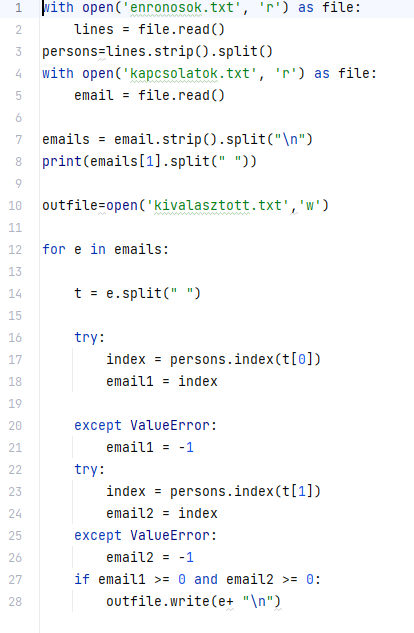
\includegraphics{images/kivalasztas}
        \caption{Szűrési művelet }    
    \end{figure}
    \begin{itemize}
        \item A fenti ábrán a program  megnyitja a 2 fájlt amelyben az adatok tárolva vannak, elsőben a személyeket tároltam, amiből tárolom egy tömbe az e-mail címeket, míg a második fájlból az üzenetek adatait fogom eltárolni .
        \item Harmadik fájlnévnél már láthatő hogy ezt fájlt nem olvasásra használom, mert ebbe fognak bekerülni a szűrésen áthaladó adatok egy része
        \item Számomra azon adatok kell hogy megmaradjanak, amelyek az első 50 személy közötti üzeneteket képezik 
        \item Ehhez a szürésnek köszönhetően elmondhatjuk hogy az 5653 felhasználóból kiválasztott első 50-hez nem 88976 üzenetet kell átnézek a következő adatvizualizációnál hanem csak 3969-et .
    \end{itemize}
    \item Második művelet ,rendezés, amely a kronológiai sorrendbe állítja az üzeneteket, kapcsolatokat, ehhez szükséges rendezést a képen látható kódrészlet által oldottam meg:
    \begin{figure}[!h]
        \centering
        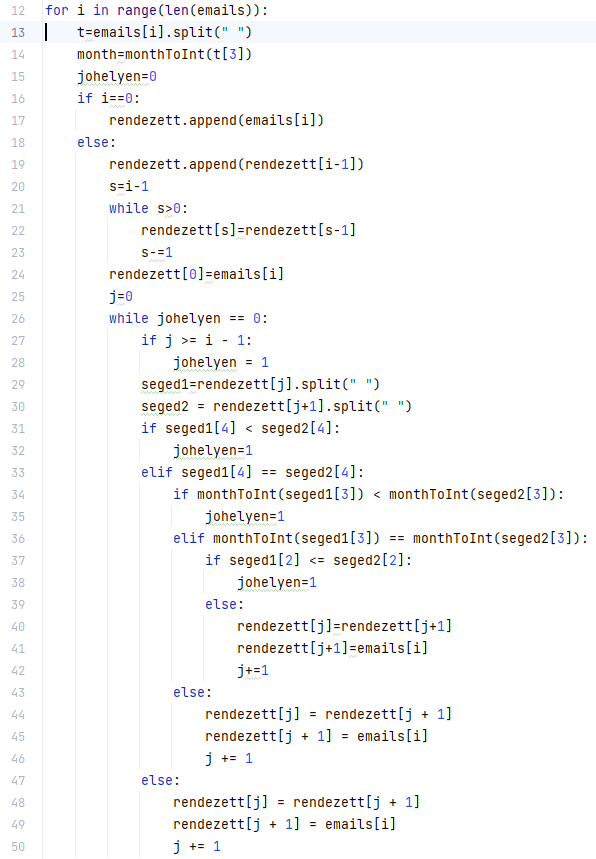
\includegraphics[scale=0.8]{images/rendezes}
        \caption{Rendezés kronológiailag}
        
    \end{figure}
    \item Az említett rendezési módszer, amit leírtál, hasznos a listaelemek sorba rendezésére. A módszeredben az elemeket egymással összehasonlítva és cserélve helyezed őket a megfelelő pozícióba. Emellett említetted, hogy egy saját függvényt használsz a hónapok helyes sorrendjének meghatározására.

Miután rendezted a listát, elmentetted az eredményt egy új fájlba, amit később felhasználhatsz az adatvizualizációhoz.

Ez a rendezési és mentési folyamat segít abban, hogy a hálózatot könnyebben áttekinthető és vizualizálható formában tudd megjeleníteni.
  
\end{itemize}
A szükséges adatcsökkentés és rendezés után következett a hálózat megjelenítése, amelyet az eddigi műveletekhez hasonló módon Pythonban készítettem el. Ez a kis rendszer egy felületet hoz létre, amely 1000 üzenet után frissíti a kapcsolati ábrát, így jól láthatók a különbségek akár 1000, akár 2000 üzenetküldés között. A rendezett e-mail lista segítségével ezek a változások idővel arányosan jelennek meg. Az alábbiakban látható a hálózat 1000 üzenet után, valamint a második képen az összes üzenet elküldése után.
\begin{figure}[h]
        \centering
        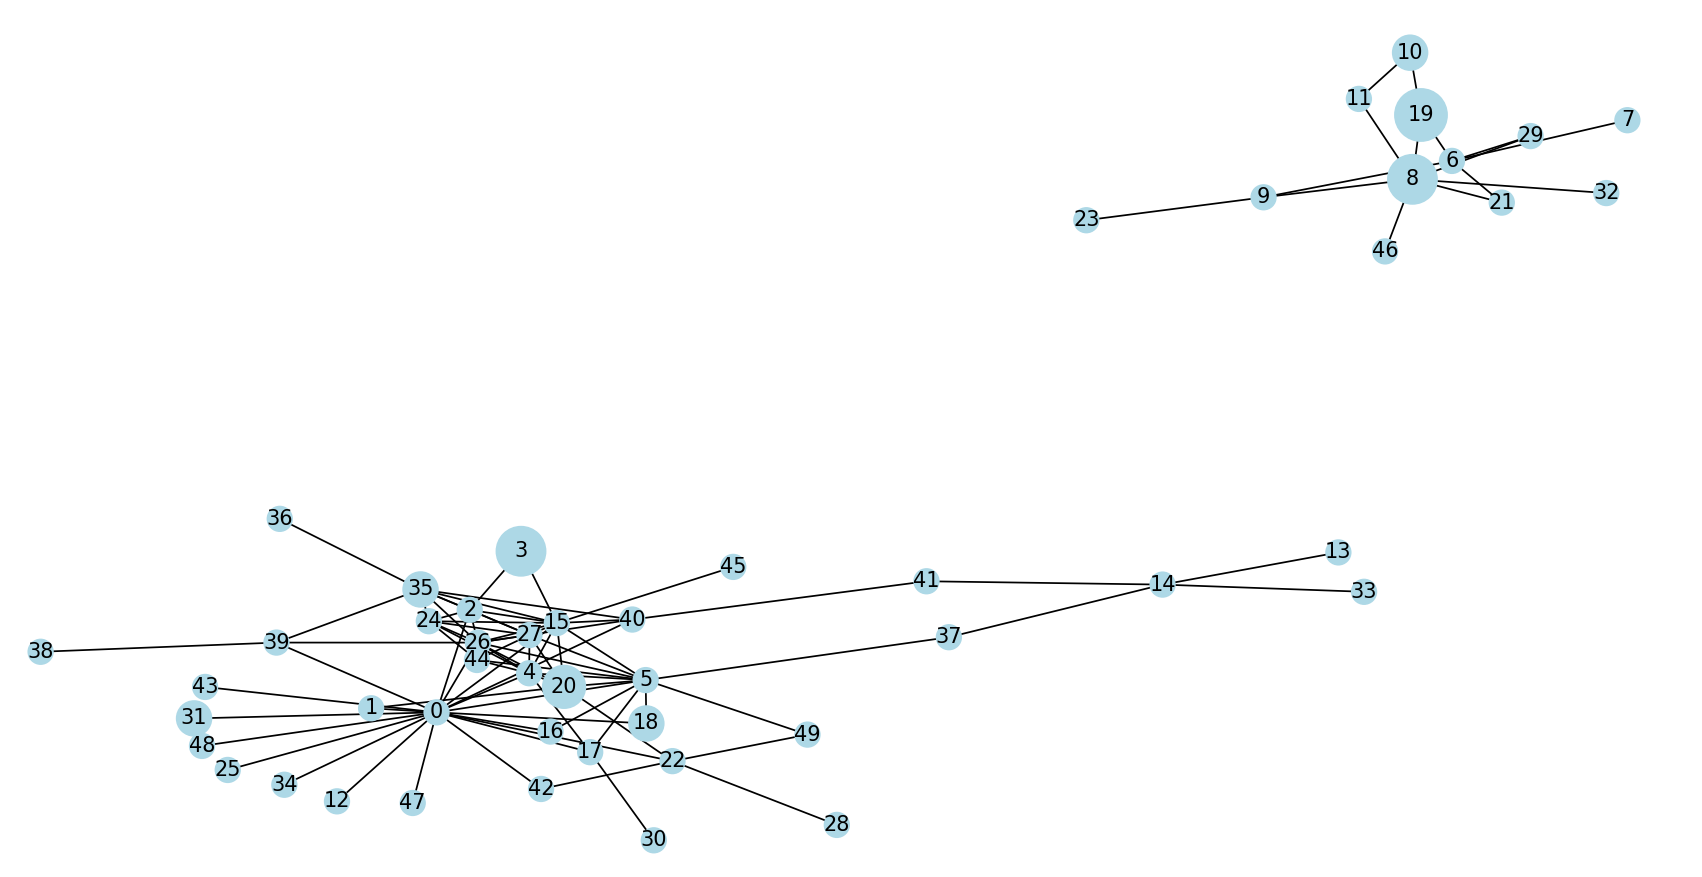
\includegraphics[scale=0.4]{images/elsorajz}
        \caption{1000 üzenet utáni hálózat}
        
    \end{figure}
    \begin{figure}[h]
        \centering
        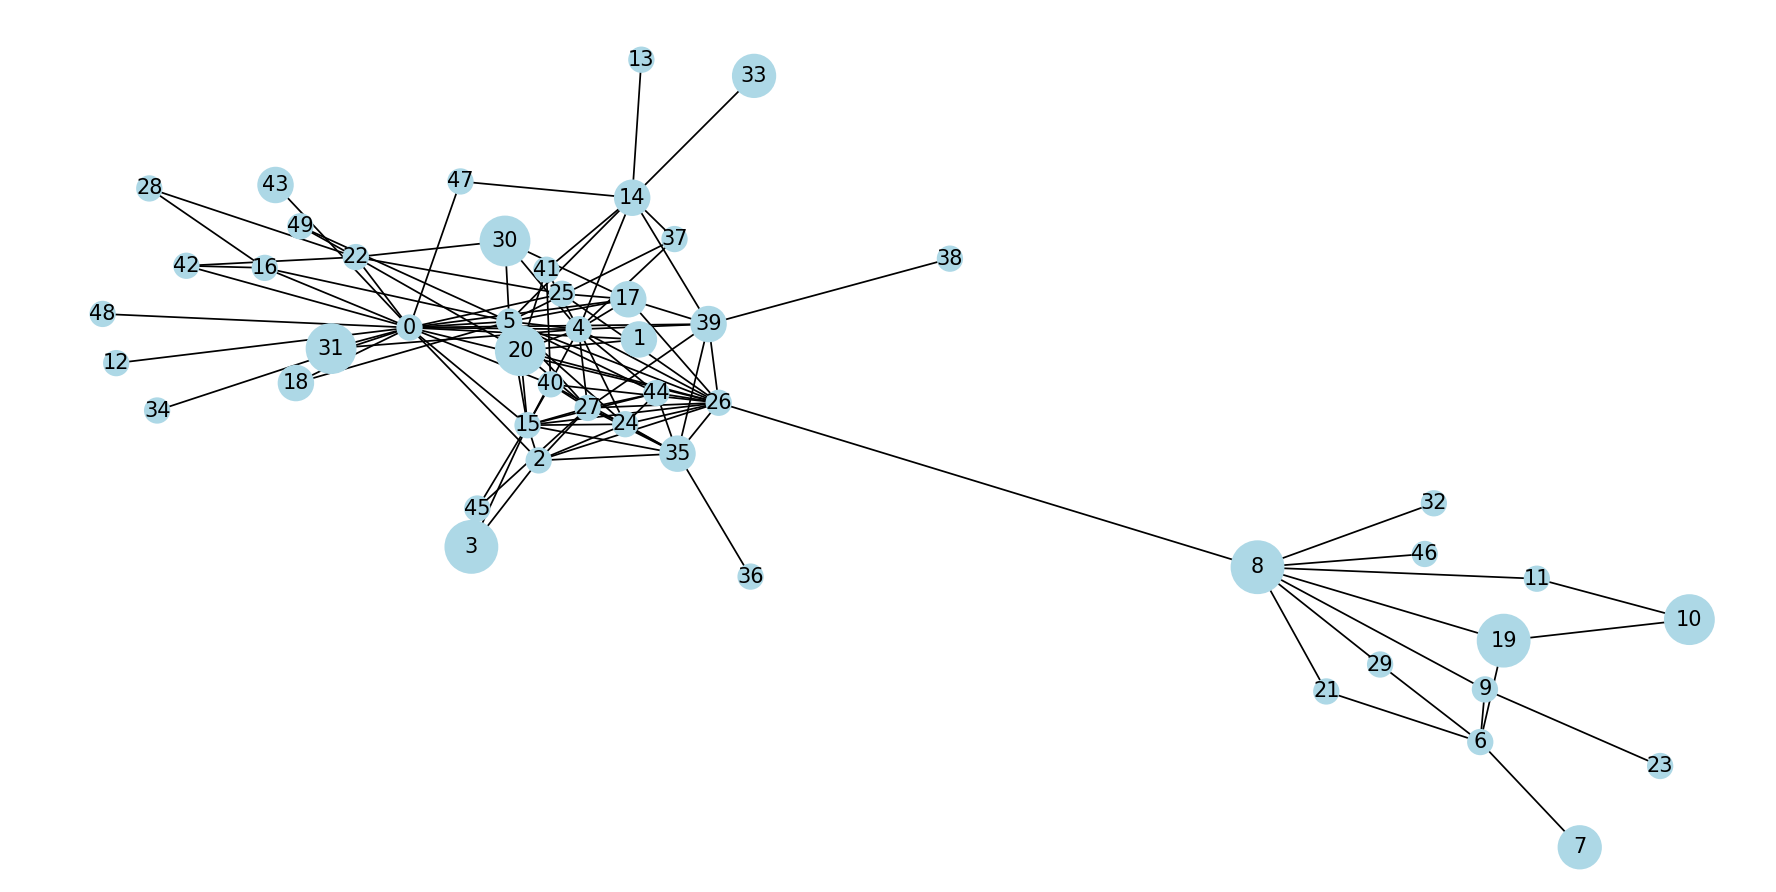
\includegraphics[scale=0.35]{images/utolsorajz}
        \caption{Összes üzenet utáni hálózat }
        
    \end{figure}

Az ábrákon észrevehető , hogy különböző méretűek a csúcspontok , amelyek az elküldött üzenetekkel arányosan növekednek .Ezen méretbeli eltérést az alábbi kód segítségével állítottam be:
\begin{figure}[h]
    \centering
    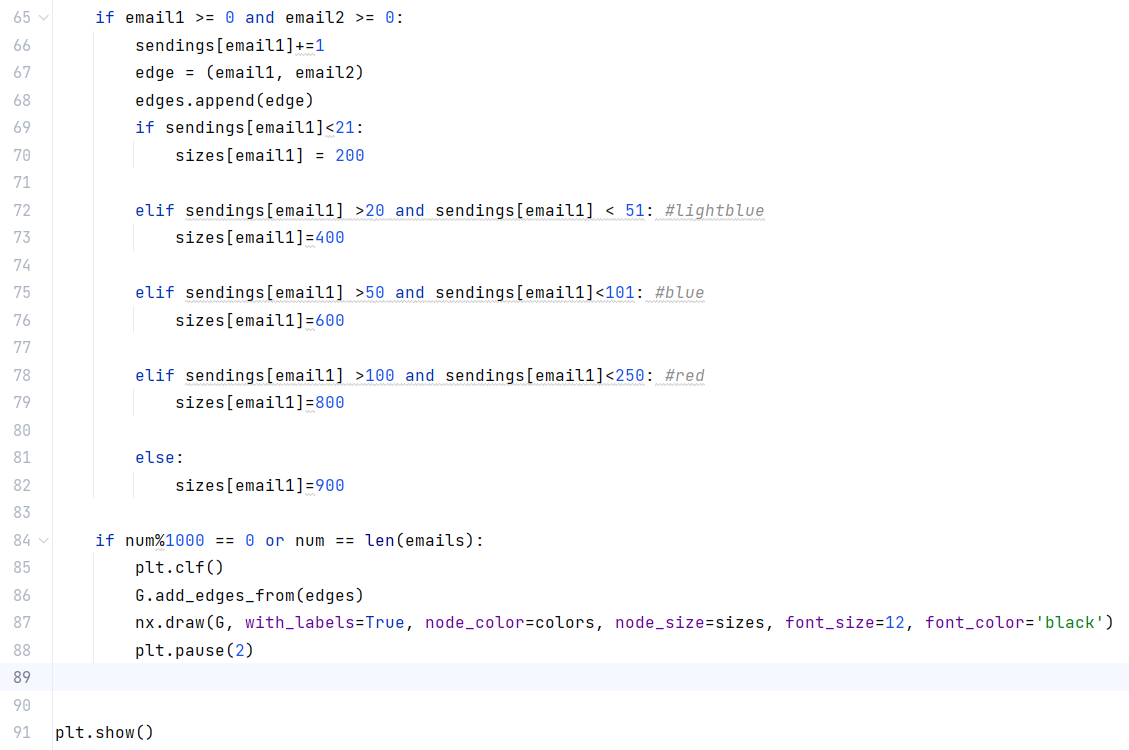
\includegraphics[scale=0.5]{images/vizualizacioskod}
    \caption{Csucspontok méretének beállítása és kijarzolása}
    \label{fig:enter-label}
\end{figure}

A kódrészletben feltüntetett 65. sorban látható egy ellenőrzés/feltétel, amelyben megnézem, hogy mindkét e-mail cím létezik-e. Ezen lépés után mindig a küldő résznél növelem az elküldött üzenetek számát, amelyet egy 50 elemű tömbben tárolok, és ezáltal tudom meghatározni, hogy az adott személy mikor kerül más területre, mikor kell növelnem az ő vizuális méretét. Ugyanakkor látható egy másik dinamikus tömb (edges névvel), amelyben számpárokat, pontosabban a gráf éleit tárolom.

Ha végeztünk az összes üzenettel, akkor a feltöltött tömbök segítségével létrehozzuk a gráfot. A tömb feltöltése több részben fog történni, mert így a kapcsolatok létrehozása során lehet kirajzoltatni a gráfot. Az általam választott lépés 1000 egységnyi nagyságú, és 2 mp-ig tart, hogy kirajzolja a gráfot, majd a következő lépés, változat következik, addig amíg eléri az utolsó üzenet feldolgozását.

Utolsó lépésként az adatvizualizációt bővítettem egy irányított gráf kirajzolásával. Az eddig használt 50 fős hálózat kapcsolatai irányokkal ellátva, valamint ráközelítve a program által generált ábra sűrített részébe.

\begin{figure}[h]
    \centering
    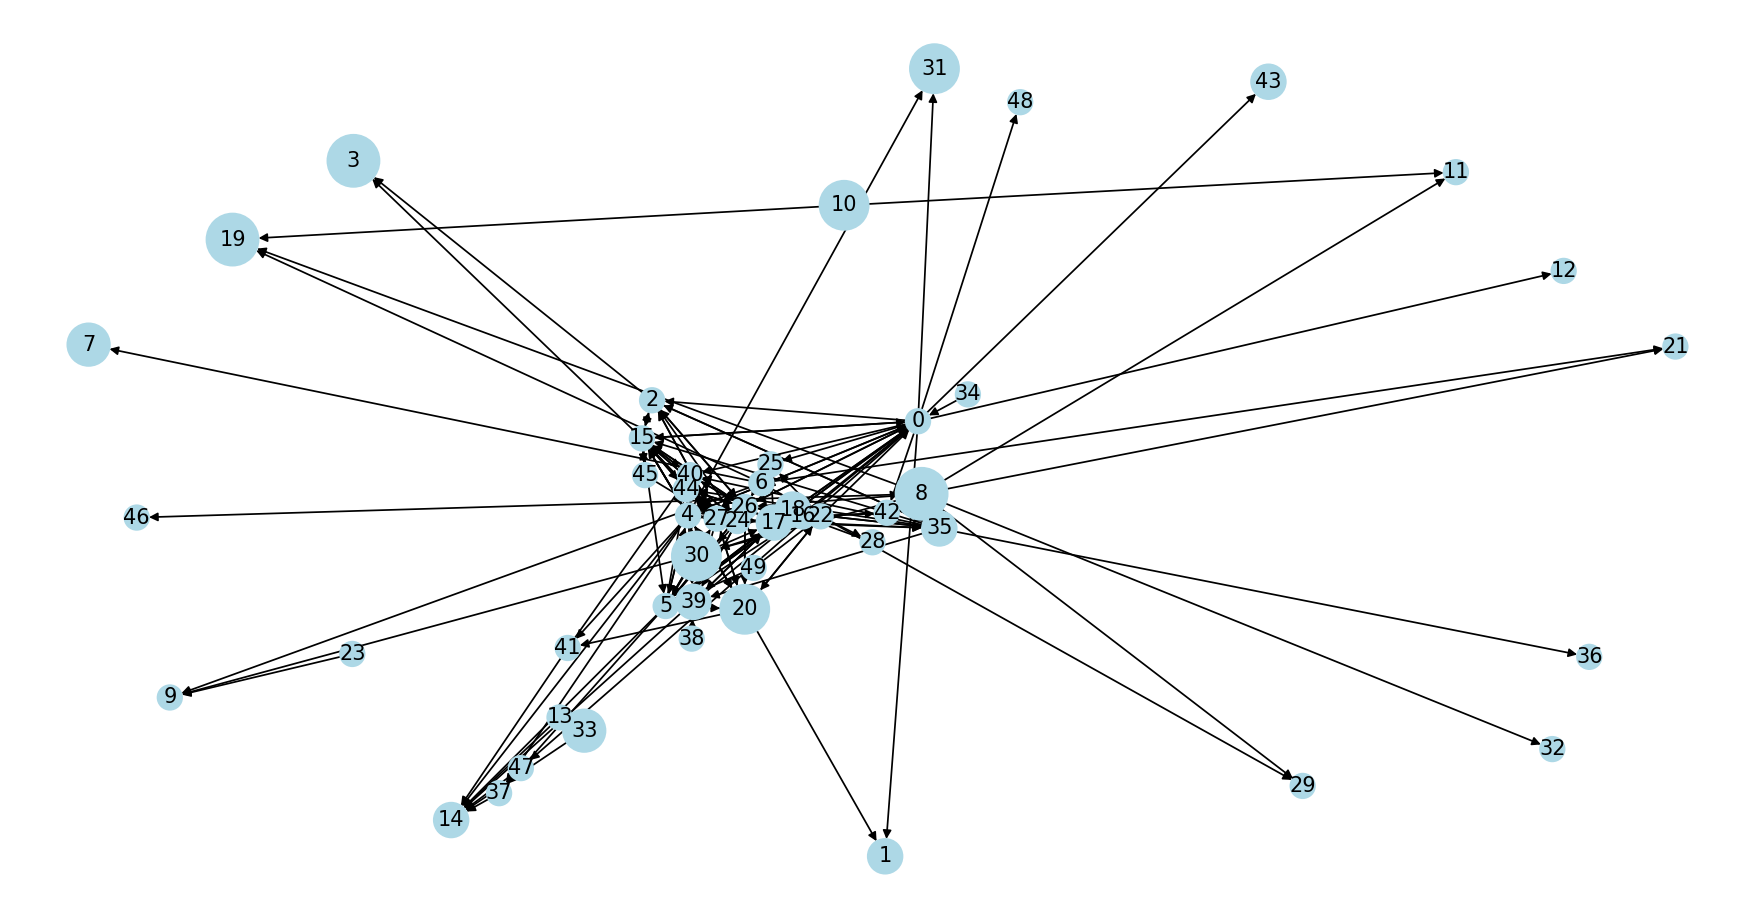
\includegraphics[scale=0.35]{images/iranyitott2}
    \caption{Csucspontok  kijarzolása irányított gráfként}
    \label{fig:enter-label}
\end{figure}
\begin{figure}[h]
    \centering
    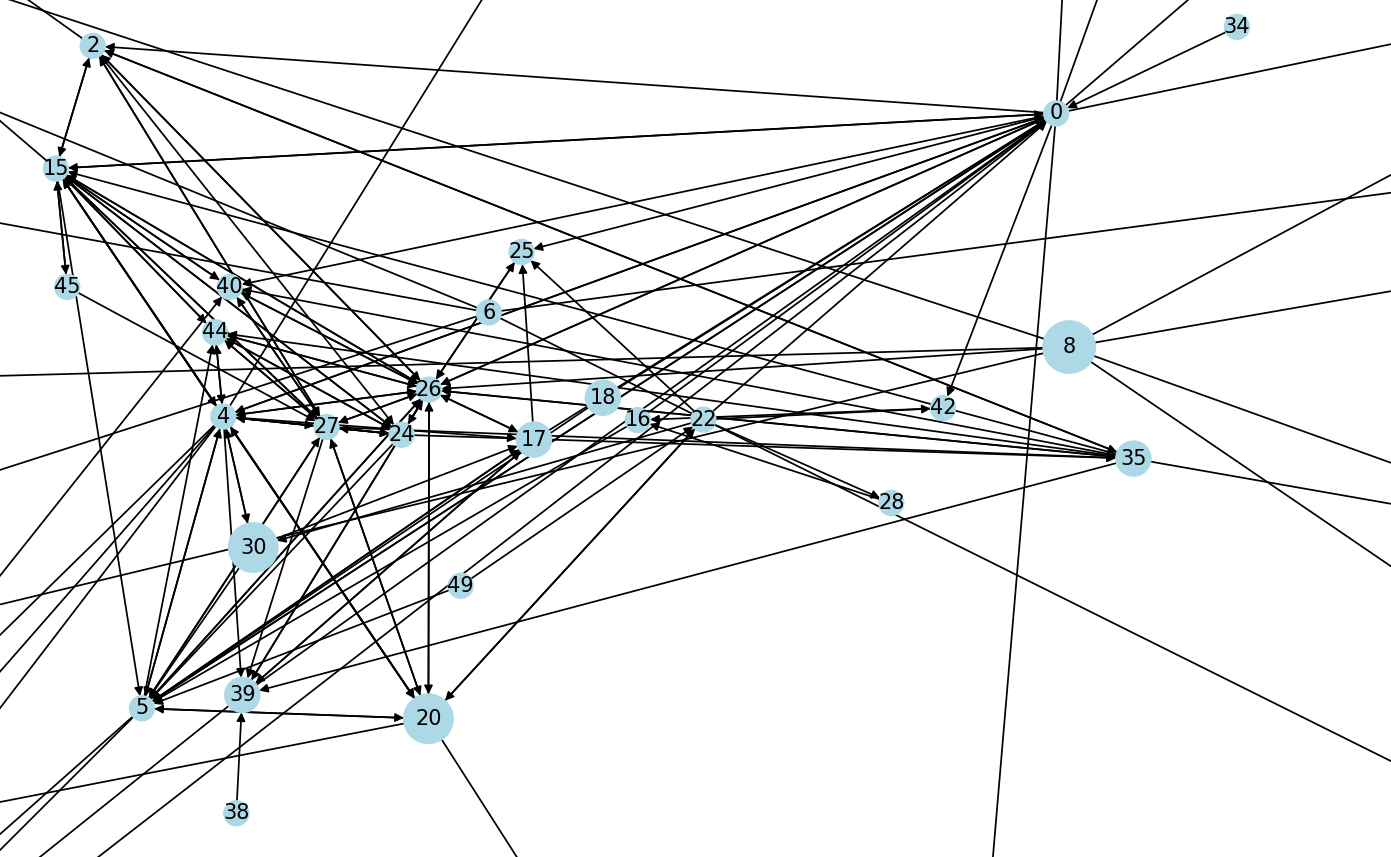
\includegraphics[scale=0.4]{images/iranyitott3}
    \caption{Kis nagyítás a gráf középpontjára}
    \label{fig:enter-label}
\end{figure}
\newpage
\section {Összességében}

A fenti esetekhez azért használtam a Python nyelvet, mert úgy éreztem, hogy ez az a nyelv, amely teljesen új volt számomra az egyetem kezdetén, valamint ezzel a nyelvvel könnyedén lehet adatokat szűrni, akár összehasonlítani egymással. Ugyanakkor nagyon sok könyvtárral rendelkezik a grafikonok vizualizációjához. Ezen könyvtárak közül választottam a Matplotlib-et, amely többek között támogatja a különböző diagramtípusokat, illetve lehetővé teszi a részletes testreszabást. Emellett nagyon elterjedt könyvtár, így rengeteg dokumentáció és példa áll rendelkezésre a különböző hibák kiküszöböléséhez.

